% Created by tikzDevice version 0.12.3.1 on 2022-05-03 12:42:51
% !TEX encoding = UTF-8 Unicode
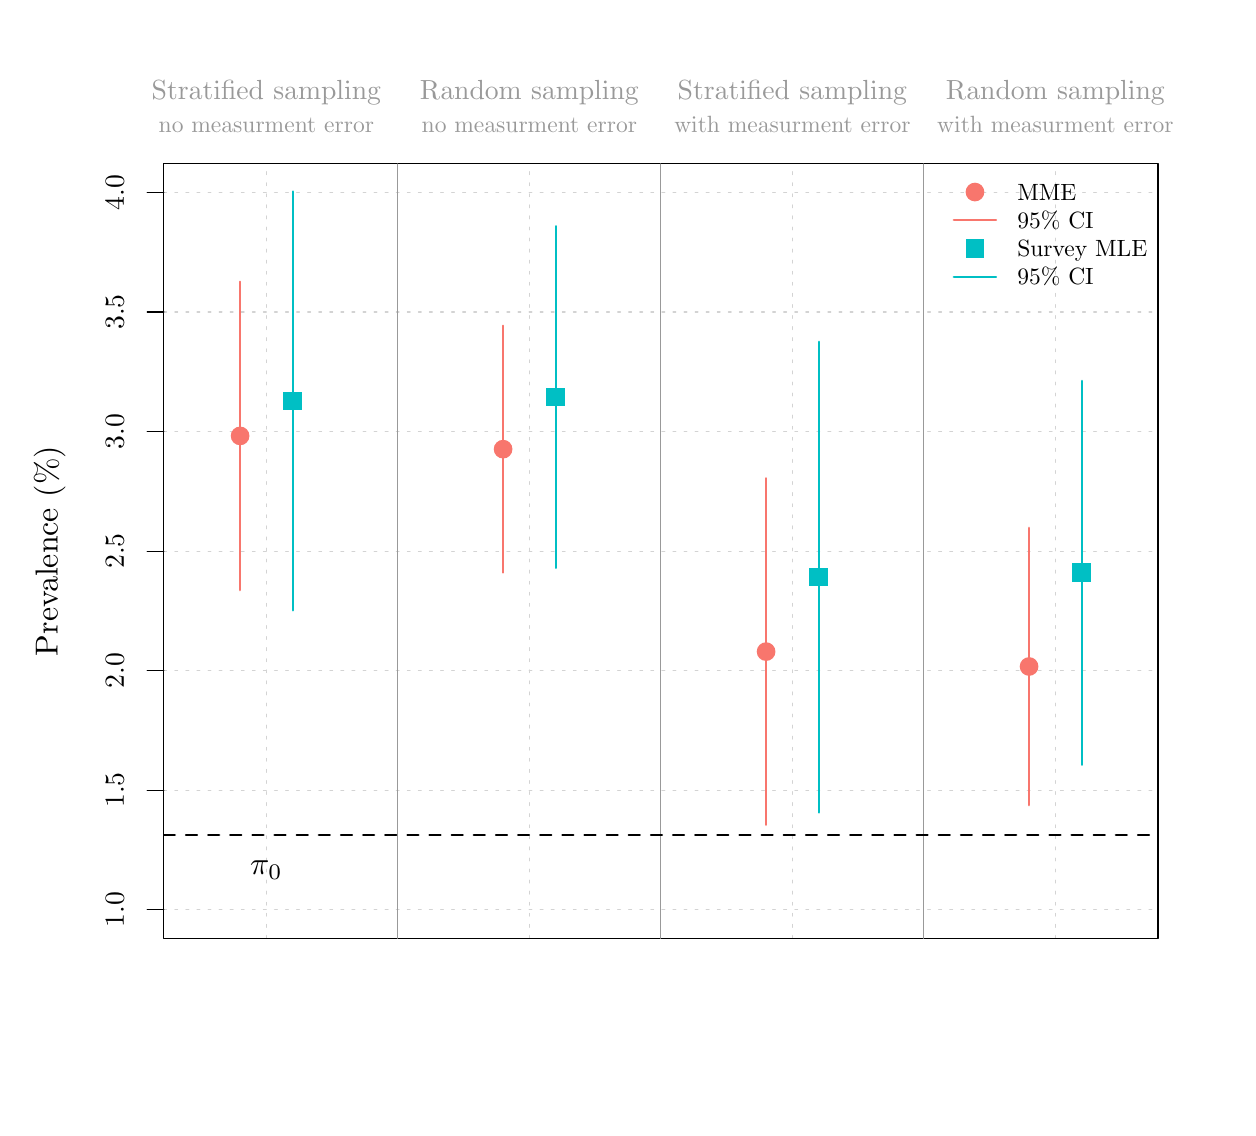
\begin{tikzpicture}[x=1pt,y=1pt]
\definecolor{fillColor}{RGB}{255,255,255}
\path[use as bounding box,fill=fillColor,fill opacity=0.00] (0,0) rectangle (433.62,390.26);
\begin{scope}
\path[clip] ( 49.20, 61.20) rectangle (408.42,341.06);
\definecolor{drawColor}{RGB}{211,211,211}

\path[draw=drawColor,line width= 0.4pt,dash pattern=on 1pt off 3pt ,line join=round,line cap=round] ( 86.26, 61.20) -- ( 86.26,341.06);

\path[draw=drawColor,line width= 0.4pt,dash pattern=on 1pt off 3pt ,line join=round,line cap=round] (133.78, 61.20) -- (133.78,341.06);

\path[draw=drawColor,line width= 0.4pt,dash pattern=on 1pt off 3pt ,line join=round,line cap=round] (181.29, 61.20) -- (181.29,341.06);

\path[draw=drawColor,line width= 0.4pt,dash pattern=on 1pt off 3pt ,line join=round,line cap=round] (228.81, 61.20) -- (228.81,341.06);

\path[draw=drawColor,line width= 0.4pt,dash pattern=on 1pt off 3pt ,line join=round,line cap=round] (276.33, 61.20) -- (276.33,341.06);

\path[draw=drawColor,line width= 0.4pt,dash pattern=on 1pt off 3pt ,line join=round,line cap=round] (323.84, 61.20) -- (323.84,341.06);

\path[draw=drawColor,line width= 0.4pt,dash pattern=on 1pt off 3pt ,line join=round,line cap=round] (371.36, 61.20) -- (371.36,341.06);

\path[draw=drawColor,line width= 0.4pt,dash pattern=on 1pt off 3pt ,line join=round,line cap=round] ( 49.20, 71.57) -- (408.42, 71.57);

\path[draw=drawColor,line width= 0.4pt,dash pattern=on 1pt off 3pt ,line join=round,line cap=round] ( 49.20,114.75) -- (408.42,114.75);

\path[draw=drawColor,line width= 0.4pt,dash pattern=on 1pt off 3pt ,line join=round,line cap=round] ( 49.20,157.94) -- (408.42,157.94);

\path[draw=drawColor,line width= 0.4pt,dash pattern=on 1pt off 3pt ,line join=round,line cap=round] ( 49.20,201.13) -- (408.42,201.13);

\path[draw=drawColor,line width= 0.4pt,dash pattern=on 1pt off 3pt ,line join=round,line cap=round] ( 49.20,244.32) -- (408.42,244.32);

\path[draw=drawColor,line width= 0.4pt,dash pattern=on 1pt off 3pt ,line join=round,line cap=round] ( 49.20,287.50) -- (408.42,287.50);

\path[draw=drawColor,line width= 0.4pt,dash pattern=on 1pt off 3pt ,line join=round,line cap=round] ( 49.20,330.69) -- (408.42,330.69);
\end{scope}
\begin{scope}
\path[clip] (  0.00,  0.00) rectangle (433.62,390.26);
\definecolor{drawColor}{RGB}{0,0,0}

\path[draw=drawColor,line width= 0.4pt,line join=round,line cap=round] ( 49.20, 61.20) --
	(408.42, 61.20) --
	(408.42,341.06) --
	( 49.20,341.06) --
	cycle;
\end{scope}
\begin{scope}
\path[clip] ( 49.20, 61.20) rectangle (408.42,341.06);
\definecolor{drawColor}{gray}{0.60}

\path[draw=drawColor,line width= 0.4pt,line join=round,line cap=round] (133.78, 61.20) -- (133.78,341.06);

\path[draw=drawColor,line width= 0.4pt,line join=round,line cap=round] (228.81, 61.20) -- (228.81,341.06);

\path[draw=drawColor,line width= 0.4pt,line join=round,line cap=round] (323.84, 61.20) -- (323.84,341.06);
\end{scope}
\begin{scope}
\path[clip] (  0.00,  0.00) rectangle (433.62,390.26);
\definecolor{drawColor}{RGB}{0,0,0}

\path[draw=drawColor,line width= 0.4pt,line join=round,line cap=round] ( 49.20, 71.57) -- ( 49.20,330.69);

\path[draw=drawColor,line width= 0.4pt,line join=round,line cap=round] ( 49.20, 71.57) -- ( 43.20, 71.57);

\path[draw=drawColor,line width= 0.4pt,line join=round,line cap=round] ( 49.20,114.75) -- ( 43.20,114.75);

\path[draw=drawColor,line width= 0.4pt,line join=round,line cap=round] ( 49.20,157.94) -- ( 43.20,157.94);

\path[draw=drawColor,line width= 0.4pt,line join=round,line cap=round] ( 49.20,201.13) -- ( 43.20,201.13);

\path[draw=drawColor,line width= 0.4pt,line join=round,line cap=round] ( 49.20,244.32) -- ( 43.20,244.32);

\path[draw=drawColor,line width= 0.4pt,line join=round,line cap=round] ( 49.20,287.50) -- ( 43.20,287.50);

\path[draw=drawColor,line width= 0.4pt,line join=round,line cap=round] ( 49.20,330.69) -- ( 43.20,330.69);

\node[text=drawColor,rotate= 90.00,anchor=base,inner sep=0pt, outer sep=0pt, scale=  1.00] at ( 34.80, 71.57) {1.0};

\node[text=drawColor,rotate= 90.00,anchor=base,inner sep=0pt, outer sep=0pt, scale=  1.00] at ( 34.80,114.75) {1.5};

\node[text=drawColor,rotate= 90.00,anchor=base,inner sep=0pt, outer sep=0pt, scale=  1.00] at ( 34.80,157.94) {2.0};

\node[text=drawColor,rotate= 90.00,anchor=base,inner sep=0pt, outer sep=0pt, scale=  1.00] at ( 34.80,201.13) {2.5};

\node[text=drawColor,rotate= 90.00,anchor=base,inner sep=0pt, outer sep=0pt, scale=  1.00] at ( 34.80,244.32) {3.0};

\node[text=drawColor,rotate= 90.00,anchor=base,inner sep=0pt, outer sep=0pt, scale=  1.00] at ( 34.80,287.50) {3.5};

\node[text=drawColor,rotate= 90.00,anchor=base,inner sep=0pt, outer sep=0pt, scale=  1.00] at ( 34.80,330.69) {4.0};
\definecolor{drawColor}{gray}{0.60}

\node[text=drawColor,anchor=base,inner sep=0pt, outer sep=0pt, scale=  1.00] at ( 86.26,364.46) {Stratified sampling};

\node[text=drawColor,anchor=base,inner sep=0pt, outer sep=0pt, scale=  0.85] at ( 86.26,352.46) {no measurment error};

\node[text=drawColor,anchor=base,inner sep=0pt, outer sep=0pt, scale=  1.00] at (181.29,364.46) {Random sampling};

\node[text=drawColor,anchor=base,inner sep=0pt, outer sep=0pt, scale=  0.85] at (181.29,352.46) {no measurment error};

\node[text=drawColor,anchor=base,inner sep=0pt, outer sep=0pt, scale=  1.00] at (276.33,364.46) {Stratified sampling};

\node[text=drawColor,anchor=base,inner sep=0pt, outer sep=0pt, scale=  0.85] at (276.33,352.46) {with measurment error};

\node[text=drawColor,anchor=base,inner sep=0pt, outer sep=0pt, scale=  1.00] at (371.36,364.46) {Random sampling};

\node[text=drawColor,anchor=base,inner sep=0pt, outer sep=0pt, scale=  0.85] at (371.36,352.46) {with measurment error};
\definecolor{drawColor}{RGB}{0,0,0}

\node[text=drawColor,rotate= 90.00,anchor=base,inner sep=0pt, outer sep=0pt, scale=  1.15] at ( 10.80,201.13) {Prevalence (\%)};
\end{scope}
\begin{scope}
\path[clip] ( 49.20, 61.20) rectangle (408.42,341.06);
\definecolor{drawColor}{RGB}{0,0,0}

\path[draw=drawColor,line width= 0.8pt,dash pattern=on 4pt off 4pt ,line join=round,line cap=round] ( 49.20, 98.39) -- (408.42, 98.39);

\node[text=drawColor,anchor=base,inner sep=0pt, outer sep=0pt, scale=  1.15] at ( 86.26, 84.24) {$\pi_0$};
\definecolor{drawColor}{RGB}{248,118,109}

\path[draw=drawColor,line width= 0.8pt,line join=round,line cap=round] (334.65,320.66) -- (349.95,320.66);
\definecolor{drawColor}{RGB}{0,191,196}

\path[draw=drawColor,line width= 0.8pt,line join=round,line cap=round] (334.65,300.26) -- (349.95,300.26);
\definecolor{fillColor}{RGB}{248,118,109}

\path[fill=fillColor] (342.30,330.86) circle (  3.38);
\definecolor{fillColor}{RGB}{0,191,196}

\path[fill=fillColor] (338.92,307.08) --
	(345.67,307.08) --
	(345.67,313.83) --
	(338.92,313.83) --
	cycle;
\definecolor{drawColor}{RGB}{0,0,0}

\node[text=drawColor,anchor=base west,inner sep=0pt, outer sep=0pt, scale=  0.85] at (357.60,327.93) {MME};

\node[text=drawColor,anchor=base west,inner sep=0pt, outer sep=0pt, scale=  0.85] at (357.60,317.73) {95\% CI};

\node[text=drawColor,anchor=base west,inner sep=0pt, outer sep=0pt, scale=  0.85] at (357.60,307.53) {Survey MLE};

\node[text=drawColor,anchor=base west,inner sep=0pt, outer sep=0pt, scale=  0.85] at (357.60,297.33) {95\% CI};
\definecolor{fillColor}{RGB}{248,118,109}

\path[fill=fillColor] ( 76.76,242.74) circle (  3.38);
\definecolor{drawColor}{RGB}{248,118,109}

\path[draw=drawColor,line width= 0.8pt,line join=round,line cap=round] ( 76.76,187.00) --
	( 76.76,298.48);
\definecolor{fillColor}{RGB}{0,191,196}

\path[fill=fillColor] ( 92.39,251.99) --
	( 99.14,251.99) --
	( 99.14,258.74) --
	( 92.39,258.74) --
	cycle;
\definecolor{drawColor}{RGB}{0,191,196}

\path[draw=drawColor,line width= 0.8pt,line join=round,line cap=round] ( 95.77,179.68) --
	( 95.77,331.05);
\definecolor{fillColor}{RGB}{248,118,109}

\path[fill=fillColor] (171.79,237.95) circle (  3.38);
\definecolor{drawColor}{RGB}{248,118,109}

\path[draw=drawColor,line width= 0.8pt,line join=round,line cap=round] (171.79,193.34) --
	(171.79,282.55);
\definecolor{fillColor}{RGB}{0,191,196}

\path[fill=fillColor] (187.42,253.39) --
	(194.17,253.39) --
	(194.17,260.14) --
	(187.42,260.14) --
	cycle;
\definecolor{drawColor}{RGB}{0,191,196}

\path[draw=drawColor,line width= 0.8pt,line join=round,line cap=round] (190.80,195.03) --
	(190.80,318.50);
\definecolor{fillColor}{RGB}{248,118,109}

\path[fill=fillColor] (266.82,164.80) circle (  3.38);
\definecolor{drawColor}{RGB}{248,118,109}

\path[draw=drawColor,line width= 0.8pt,line join=round,line cap=round] (266.82,102.18) --
	(266.82,227.43);
\definecolor{fillColor}{RGB}{0,191,196}

\path[fill=fillColor] (282.45,188.34) --
	(289.20,188.34) --
	(289.20,195.09) --
	(282.45,195.09) --
	cycle;
\definecolor{drawColor}{RGB}{0,191,196}

\path[draw=drawColor,line width= 0.8pt,line join=round,line cap=round] (285.83,106.67) --
	(285.83,276.75);
\definecolor{fillColor}{RGB}{248,118,109}

\path[fill=fillColor] (361.85,159.42) circle (  3.38);
\definecolor{drawColor}{RGB}{248,118,109}

\path[draw=drawColor,line width= 0.8pt,line join=round,line cap=round] (361.85,109.30) --
	(361.85,209.53);
\definecolor{fillColor}{RGB}{0,191,196}

\path[fill=fillColor] (377.49,189.90) --
	(384.24,189.90) --
	(384.24,196.65) --
	(377.49,196.65) --
	cycle;
\definecolor{drawColor}{RGB}{0,191,196}

\path[draw=drawColor,line width= 0.8pt,line join=round,line cap=round] (380.86,123.91) --
	(380.86,262.64);
\end{scope}
\end{tikzpicture}
